\chapter{Related Work}
\label{chapter:related_work}
This chapter will introduce relevant publications regarding dental caries detection, focusing mainly on detection from bitewing radiographs. Following that, we will briefly introduce methods for the segmentation of dental restorations.

\section{Dental caries detection}
Since 2017, more than ten publications have been released regarding automatic caries detection from images \cite{PradosPrivado2020}. They differ in how they approach caries localization and the types of images they use. The following images have been used: Near-Infrared Transillumination images \cite{Casalegno2019,Schwendicke2020}, camera photographs \cite{Moutselos2019}, and X-ray images, which may be further classified into bitewing \cite{Moran2021, Cantu2020, Bayrakdar2021, Mao2021, Srivastava2017}, panoramic \cite{Lian2021}, and periapical X-ray images \cite{Lee2018}.

All the related publications can be divided into three groups based on their approach to caries localization: Manual detection and classification, dental caries segmentation, and dental caries detection.

\subsection{Manual detection and classification}
This section introduces publications that approached caries detection in the following manner: First, they crop individual teeth from the X-ray image, using manual cropping or non-machine learning computer vision techniques. After the tooth is extracted from the image, it is labeled by a professional. A classifier is trained on those image patches to decide if it contains a carious lesion.
\begin{itemize}
    \item First attempts to use a neural network for caries detection date back to 2008, when Kuang et al. \cite{Kuang2008} proposed an approach based on passing a patch from an image to a classifier, which then decided if the patch contains caries or healthy enamel. Even though the performance of the proposed neural network was surpassed by 6.72\% by kernel SVM, it was still able to outperform an ordinary dentist by more than 5\%. It was only 6\% worse than an experienced individual.
    \item Moran et al.\cite{Moran2021} used histogram equalization, Otsu's thresholding, and morphological operations to extract individual teeth from bitewing images. After the teeth had been cropped from the image, the dataset was labeled by assigning one of three categories to each tooth. The categories were: Normal teeth, incipient lesions, and advanced lesions. Moran et al. processed a total of 112 radiographs this way, resulting in 480 teeth with corresponding annotations. They trained the ResNet and Inception model to perform the classification task, and the best-achieved accuracy was 73.3\% \cite{Moran2021}.
    \item{Mao at al. \cite{Mao2021}} made a similar preprocessing approach as Moran, only this time extracting unilateral tooth images instead of the whole tooth. A total of 3716 images of unilateral teeth were obtained. AlexNetsed was used for classification and reached a 90.3\% accuracy.
    \item{Lee et al. \cite{Lee2018}} published a similar approach, however, with periapical images. A dataset with 3000 images was created manually by cropping out teeth from the X-ray image, keeping only those without extensive dental restorations. Two teeth at once were also extracted from the radiograph in the same process. After obtaining this dataset, they trained GoogLeNet and Inception v3 architecture classifiers, reaching an accuracy of 89\%  for molars and 82\% for images with both premolars and molars.
\end{itemize}


\subsection{Dental caries segmentation}
There are publications where the authors approached the task of caries localization as semantic segmentation. The advantage of this approach is the pixel precision of the lesion detection. On the other hand, creating a similar dataset is very time-consuming. An example of a dataset annotated in a pixel-wise manner is depicted in Figure \ref{fig:segmentation_lit} as well as predictions of a model proposed by Cantu \cite{Cantu2020}.

\begin{figure}
    \centering
    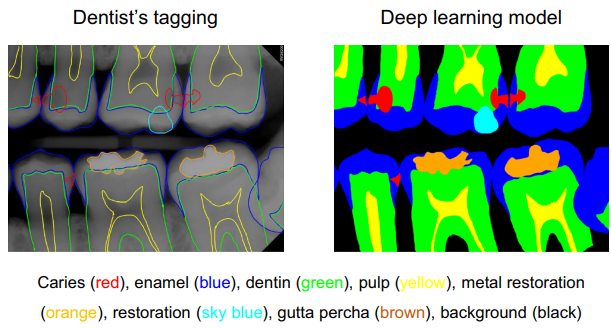
\includegraphics[width=\linewidth]{images/segmentation_bitewing_rich.png}
    \caption{Annotated bitewing radiograph and the same image post-processed, source \cite{Lee2021}}
    \label{fig:bitewing_dense}
\end{figure}

\begin{itemize}
    \item{Cantu et al. \cite{Cantu2020}} created a dataset of 3686 bitewing images. Three dentists drew a polygonal-shaped box over caries independently in each image. In the case of a unanimous decision, the annotation was kept in the dataset. Otherwise, the fourth dentist reviewed the annotation and decided if it should be kept or deleted. Cantu et al. used the U-Net model with EfficientNet B5 as a backbone. They then evaluated the model per pixel, and its performance was compared against seven dentists, outperforming their mean performance in every metric.
    \item{Lian et al. \cite{Lian2021}} chose the same approach as Cantu but used panoramic images. In comparison with Cantu, following the segmentation, they cropped the region of interest around the segmented lesion and classified caries into one of four categories as described in Section \ref{sec:caries_classification}. They achieved an IOU score of 0.785 on the segmentation task. In comparison, the best performing dentist achieved an IOU of 0.717. In the classification task, the model outperformed the average dentist's performance.
    \item {Lee et al. \cite{Lee2021}}  approached the problem uniquely. Their dataset, consisting of 304 bitewing radiographs, was densely annotated by polygons, denoting the position of dental caries, enamel, dentine, pulp, and gutta-percha restorations. The result of this annotation can be seen in Figure \ref{fig:bitewing_dense}. They used two independent U-net models to predict the position of caries and remaining structures in the image. The output of both models was post-processed and merged. Even though the model achieved an F1 score of 0.641, which is low compared to other publications, predictions of the model helped dentists improve their sensitivity ratio by 7 - 10\%.
\end{itemize}

\begin{figure}
    \centering
    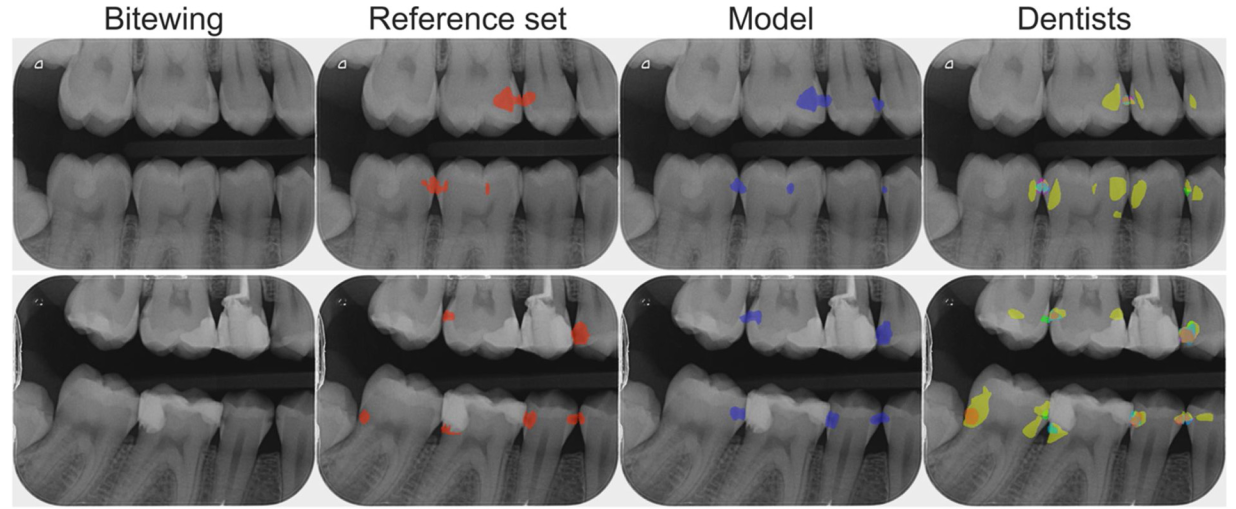
\includegraphics[width=\linewidth]{images/segmentatic_literature.png}
    \caption{Sample of data and predictions of the model by }
    \label{fig:segmentation_lit}
\end{figure}

\subsection{Dental caries detection}
\begin{figure}
    \centering
    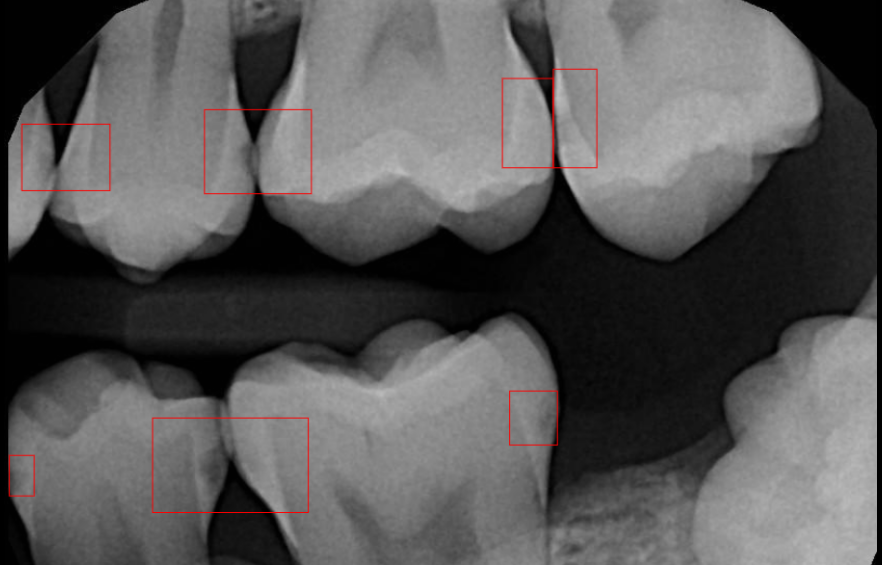
\includegraphics[width=\linewidth]{images/sirvastava_pred.png}
    \caption{Predictions of the model proposed by Srivastava et al., source \cite{Srivastava2017}}
    \label{fig:srivastava_preds}
\end{figure}
\begin{itemize}
    \item{Srivastava et al. \cite{Srivastava2017}} trained a fully convolutional neural network with over 100 layers on a dataset containing more than 3000 bitewing radiographs. They denoted the position of tooth decay in a pixel-wise manner. Even though the model predicts output masks in a semantic segmentation fashion, the output is post-processed by fitting a minimal bounding rectangle around the prediction, as can be seen in Figure \ref{fig:srivastava_preds}. After that, the model is evaluated by computing the IOU of the rectangle with the ground truth polygon. If the IOU is greater than 0.8, the detection is considered positive. Srivastava et al. claim that their model considerably outperforms each of the three dentists included in the study. Detailed results are in Table \ref{tab:srivastava_results}.

          \begin{table}
              \centering
              \begin{tabular}{c||c|c|c|c|c}
                  Metric    & Model \cite{Srivastava2017} & Model \cite{Kumar2018} & Dr. 1 & Dr. 2 & Dr. 3 \\ \hline
                  Recall    & 0.805                       & 0.70                   & 0.477 & 0.433 & 0.344 \\ \hline
                  Precision & 0.615                       & 0.53                   & 0.63  & 0.815 & 0.891 \\ \hline
                  F1-Score  & 0.70                        & 0.614                  & 0.54  & 0.56  & 0.50
              \end{tabular}
              \caption{Results of models proposed in \cite{Srivastava2017} and \cite{Kumar2018}, compared with three dentists, modified}
              \label{tab:srivastava_results}
          \end{table}

    \item{The same author and Kumar \cite{Kumar2018}} published another paper, where they changed the model to U-Net, which was trained on an extended dataset of 6000 bitewing X-ray images. The authors tested the hard example mining approach, but it led to a decrease in performance. Even though U-Net architecture usually achieves better results on publicly accessible benchmarks \cite{paperwithcode, Zhang2019}, and the size of the dataset increased twofold, the model's performance dropped by 15\%, see Table \ref{tab:srivastava_results}. There is no information available about the evaluation protocol used by Kumar \cite{Kumar2018}, nor about the IOU threshold needed to consider a prediction to be correct. This makes it hard to estimate the cause of the performance drop.
    \item{Barakdar et al. \cite{Bayrakdar2021}} did both semantic segmentation and object detection with a dataset of 621 bitewing images available for both of those tasks. They claim to use U-net for segmentation and VGGNet for object detection. However, the paper does not mention how they modified the VGGNet architecture for object classification to perform an object detection task. The object detection results were evaluated against five professionals in dentistry with different years of experience. The model outperformed two dentists with two and three years of experience while being outperformed significantly by all three dentists with ten years of experience. The reported precision of the model is $0.78$, recall=$0.77$ and F1 score of $0.78$. No information about the overlap used to consider predictions to be correct is included in the paper. We assume it was set to be $0.5$.
    \item{Bayraktar et al. \cite{Bayraktar2021}} solved only the object detection task on a dataset of 1000 bitewing images labeled by two experts with more than ten years of experience. With YOLOv3 architecture model, they achieved $AP@.5 = 0.872$ .
\end{itemize}

\section{Dental restorations segmentation}
\label{sec:related_works:dental_restorations}
To the author's knowledge, there are no available publications regarding the segmentation of dental restorations in bitewing radiographs. Therefore, we will introduce two methods that segment dental caries from panoramic X-ray images. Figures \ref{fig:restoration_seg_pub1}, \ref{fig:restoration_seg_} contain samples of images used for restoration segmentation.
In addition, we will mention two publications where restoration detection was a minor part of the work.
\begin{figure}
    \begin{floatrow}[2]
        \ffigbox[1.25\FBwidth]{\caption{Results of segmentation algorithm proposed by Yeshua et al.\cite{Yeshua2019}}\label{fig:restoration_seg_pub1}}%
        {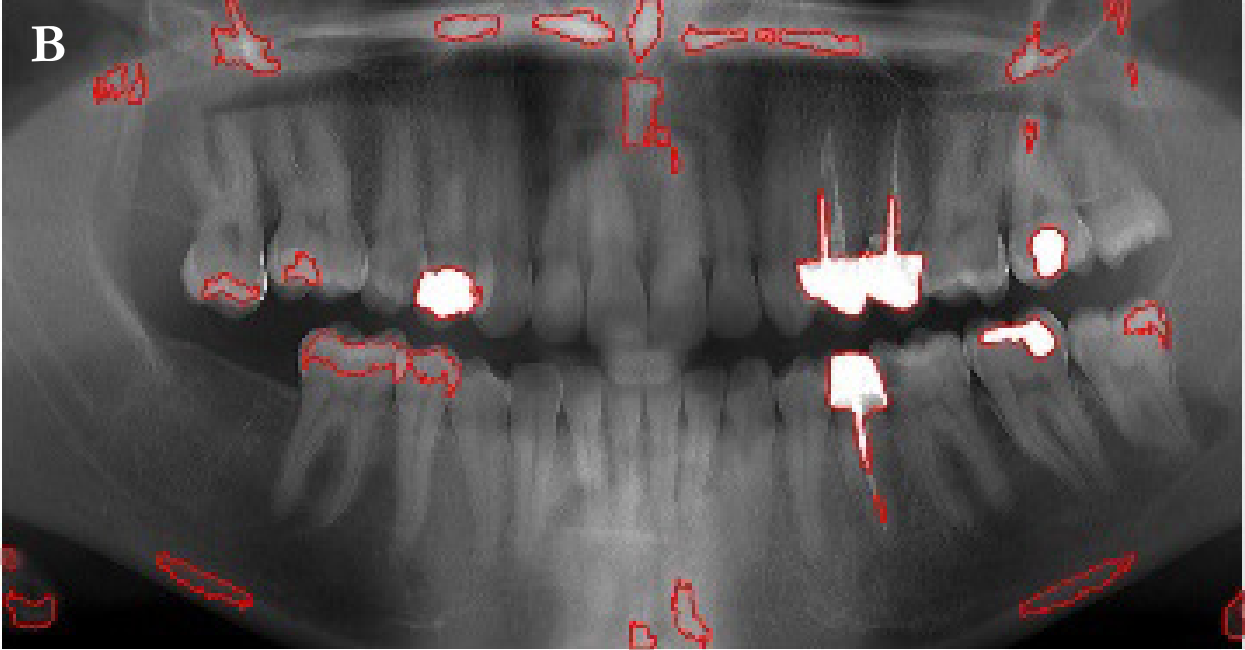
\includegraphics[width=\linewidth]{images/segmentation_opg.png}}\;
        \ffigbox[0.75\FBwidth]{\caption{Cropped region from panoramatic image with multiple restorations, source \cite{AbdallaAslan2020}}\label{fig:restoration_seg_pub2}}%
        {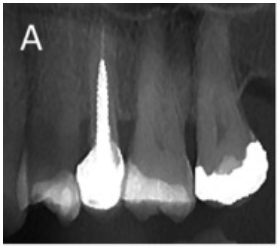
\includegraphics[width=\linewidth]{images/segmentation_crop.png}}
    \end{floatrow}
\end{figure}
\begin{itemize}
    \item{Mao et al. \cite{Mao2021}} classified dental segmentations in previously extracted image patches with unilateral teeth.
    \item{Lee et al. \cite{Lee2021}} did not focus directly on the segmentation of restorations, yet it was one of the classes segmented out by their U-net architecture. There are no metrics available regarding the algorithm's performance on dental restorations.
    \item{Abdalla-Aslan et al. \cite{AbdallaAslan2020}} used methods of classical computer vision to segment out restorations in panoramic images. Their pipeline consisted of: Adaptive gaussian thresholding, morphological operations, and deleting regions in peripheral areas of the image. The final algorithm had the precision and sensitivity of 0.33 and 0.946, respectively. After successful detection, the restoration was classified as: dental implant, crown, amalgam filing, etc.
    \item {Yeshua et al. \cite{Yeshua2019}} solved the same problem as Abdalla-Aslan. Even the approach was more-less the same, except theirs achieved a precision of 0.568. They classified detected areas similarly to Abdalla-Aslan, having an extra category for false detections. After the removal of false detections, the precision was boosted to 0.98.
\end{itemize}